\section{Warum Git}

\begin{frame}{Was brauchen wir?}
	\begin{block}{Das Problem}
		Dateien zwischen Machine synchronisieren und sie mit mehr Leute
		bearbeiten. Spezifischer Textdateien bearbeiten (z.B. Quellcode)
	\end{block}
	\pause

	\begin{block}{Eine L\"osung}
	\centering
	\vspace{1em}
	\includegraphics[width=0.25\textwidth]{pic/git.png}\\
	\vspace{1em}

	(Engl. f\"ur Bl\"odmann) Entwickelt von Linus Torvalds
	\end{block}
\end{frame}

\begin{frame}{Was ist git?}
	\begin{block}{Was wir brauchen}
	\begin{itemize}
		\item Synchronisation
		\item Team Datei Bearbeitung
		\item Problemlose Offline-Nutzung
	\end{itemize}
	\end{block}
	\pause

	\begin{block}{Was kriegen wir extra}
	\begin{itemize}
		\item Geschichte jedes Dokuments im Projekt
		\item Kryptographische Sicherheit der Projektgeschichte
		\item Gemeinsamer Dateizugriff ohne zentraler Server 
	\end{itemize}
	\end{block}
\end{frame}

\begin{frame}[c]{Bemerkung}
	\centering
	{\LARGE 
	Git l\"ost ein komplex Problem \\
	daher ist Git auch komplex
	}

	{\footnotesize
		But don't worry it's not \emph{too} hard
	}
\end{frame}

\section{Git lernen}

\begin{frame}{Begriff: Repository}
\end{frame}

\begin{frame}{Snapshots}
    \begin{center}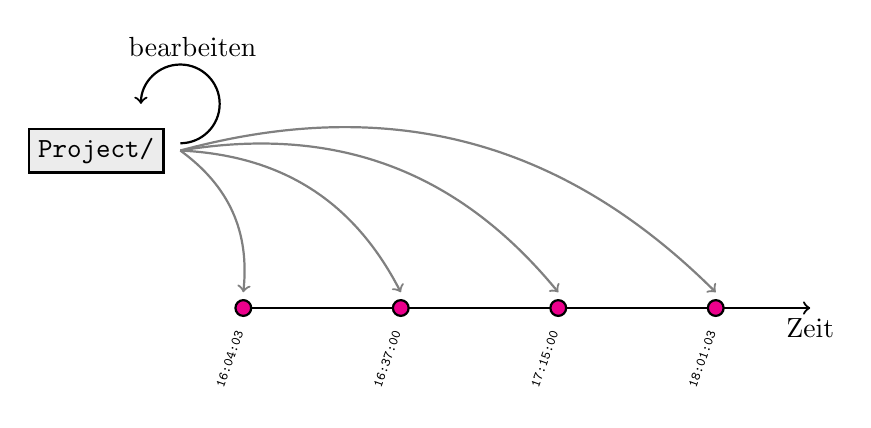
\begin{tikzpicture}
    \node at (-1, 2) [draw, fill=gray!15, thick, font=\ttfamily, left] (P) {Project/};
    \pause
    \draw[black, thick, ->] (P.north east) ++(.2,-.2) arc (-90:180:.5)
        node[pos=.6, above]{bearbeiten};
    \draw[black, thick, ->] (0, 0) -- (7.2, 0) node [below] {Zeit};
    \foreach \x/\t in {0/16:04:03, 2/16:37:00, 4/17:15:00, 6/18:01:03}
    {
        \pause
        \draw[color=black, fill=magenta, thick] (\x, 0) circle (.1)
            node[below=5pt, anchor=east, rotate=70, font=\ttfamily] {\tiny \t};
        \draw[thick, ->, gray] (-.8, 2) to[bend left] (\x, .2);
    }
    \end{tikzpicture}\end{center}
\end{frame}

\begin{frame}{Begriff: Commit}
    \begin{block}{Ein Commit enthalt}
    \begin{itemize}
        \item Die \"Anderungen der Dateien \pause
        \item Autor Name + Email \pause
        \item Zeitstempel \pause
        \item \textbf{Eine Beschreibung der \"Anderungen} \pause
        \item kryptographisches Hash der Dateien \pause
    \end{itemize}   
    \end{block}
\end{frame}

\begin{frame}[fragile]{Commit Beispiel}
    \centering\footnotesize
    \begin{verbatim}
commit e584e04c5f8ffb14e50c701c1fd8178457a51743
Author: Nao Pross <naopross@thearcway.org>
Date:   Tue Jan 22 04:31:30 2019 +0100

    Add test for task and job, fix bug in job

    By being a std::set job did not allow to add duplicate
    elements, changing it to a std::multiset fixes the issue.

    \end{verbatim}
\end{frame}

\begin{frame}{Begriff: Remote}
\end{frame}

\begin{frame}{Begriff: Merge}
\end{frame}

\begin{frame}{Begriff: Fork}
\end{frame}

\section{Git benutzen}



\begin{frame}{Arbeitsablauf}
	Arbeitsablauf um eine Formelsammlung zu bearbeiten (alleine).
	\begin{enumerate}
		\item Fork ein Repository von HSR-Stud \pause
		\item Bearbeiten \pause
		\item Fortlaufend Commits erstellen Bsp. nach jedem Kapitel \pause
		\item Push
	\end{enumerate}
	
\end{frame}

\begin{frame}{Arbeitsablauf II}
Arbeitsablauf um eine Formelsammlung zu bearbeiten (mehrere Autoren).
\begin{enumerate}
	\item Fork ein Repository von HSR-Stud  \pause
	\item Jede Person erstellt einen Branch \pause
	\item Bearbeiten \pause
	\item Fortlaufend Commits erstellen Bsp. nach jedem Kapitel \pause
	\item Mit dem Master mergen Bsp. nach jedem Kapitel \pause
	\item Push
\end{enumerate}

\end{frame}
